%% The comment character in TeX / LaTeX is the percent character.
%% The following chunk is called the header

\documentclass{article}	% essential first line
\usepackage{times}		% this uses fonts which will look nice in PDF format
\usepackage{graphicx}		% needed for the figures
\usepackage{url}
\usepackage{adjustbox}
\usepackage{amsmath}
\usepackage{listings}
\usepackage{multicol}
\usepackage{color}
\usepackage{multirow}
\usepackage{array}

%% Set the folder where pictures are located
\graphicspath{ {images/} }

%% Here I adjust the margins

\oddsidemargin -0.5in%-0.25in		% Left margin is 1in + this value
\textwidth 7.5in		% Right margin is not set explicitly
\topmargin 0in			% Top margin is 1in + this value
\textheight 9in			% Bottom margin is not set explicitly
\columnsep -0.25in %0.25in		% separation between columns

% set listing settings
\lstset{language=C, 
		numbers=left,
		frame=single,
		tabsize=2,
		breaklines=true,
		commentstyle=\color{red}}

%% Define the fields to be displayed by a \maketitle command
\author{Dee, Timothy\\
    \texttt{timdee@iastate.edu}
    \and
    Long, Justin\\
    \texttt{jlong@iastate.edu}
    \and
    McDonnel, Brandon\\
    \texttt{bmcdonnel@iastate.edu}
}

\title{Remotely Connected Electric Field Generator\\
for Particle Separation in a Fluid \\
\large{Team May1612}}

%%
%% Header now finished
%%

\begin{document}		% Critical
\thispagestyle{empty}		% Inhibit the page number on this page
\maketitle			% Use the \author, \title and \date info

\begin{multicols}{2}

\abstract{
This document details the design and implementation of a
remotely connected electric field generator.
The goal of this design is to provide an easy interface for
manipulating the output voltage and frequency of a circuit
remotely in order to generate an electric field.
This electric field,
when applied to a fluid over a long period of time
will cause particles in the fluid to separate.
The hardware and software components used to accomplish
the aforementioned goal are described in detail.
}

% Make an argument for why this project is:
% useful
% necessary
% novel
\section{Introduction}
New research has shown that certain particles may be separated from fluids through dielectrophoresis.
This process involves applying an electric field to a fluid.
The field may be manipulated in order to attract or repel certain particles.
The particles the electric field will attract or repel depends on
characteristics of the electric filed which may be controlled
by varying the voltage and frequency of the electronics driving the field.

This technology has many useful applications in health care
% TODO

\section{Project Definition}
In our implementation, an electric field is applied 
to two metal plates.
by varying the voltage and frequency
applied to these plates, 
the properties of the electric field can be changed.

Our job is to construct a system 
containing an electronic circuit capable of providing
the necessary voltages and frequencies required 
to drive a pair of metal plates.
This system must enable the circuit to be controllable 
through the use of a web interface.
In addition, a small form factor must be maintained.

The system must be able to generate up to a 60 V peak-peak sine wave with
user-controlled variable frequency from 10 kHz to 1 MHz. 
% TODO

\section{Deliverables}
There are four items which must be constructed for this project:
% TODO list the components which must be constructed

For the analog circuit components,
functionality of the circuit will be tested
using an oscilloscope to verify 
the requirements have been satisfied.
This method can also be used to ensure 
the output signal contains minimal amounts of noise and distortion. 

% TODO if we don't get to the research component of the project,
% we should remove this
The construction of this device is the first phase of the project.
After the completion of this component,
the device will be used 
to experiment with particle separation in various fluid types.
These experiments constitute the remainder of the project.
% TODO add adam's name
For these experiments our advisor at Minetronix, John Pritchard, 
will be the main source of guidance and testable material. 

\section{Constraints}
Constraints on this project fall within the size, voltage, and portability domains.

The size requirements of this project are directly related 
to the portability of the final design.
The design requirements specify this system must be easily and quickly
 moved around from one workstation to another.
The maximal allowed size is approximately 
the size of a backpack 
with smaller sizes being more desirable
but not explicitly required.
With the electronics currently being used,
these requirements will easily be met.

Another constraint arises from the power supply requirements.
The power supply must deliver at least 60V DC in order to feed the amplifier circuit. 
Due to this, the final design requires a power brick
similar to one which would be used to charge a laptop.
Importantly, this would require the device to be plugged into a wall outlet.
This is not seen as an issue.
Every location this device will operate 
will most likely have other equipment with similar power requirements.

In order to use this system,
there are other items which are required
apart from the device itself. 
The first requirement is a network connection between the device and a computer.
This connection is necessary to be able to interact with the web server hosted on the Raspberry Pi. 
Without a computer to interact with this system there is no practical means of utilizing the device's functionality. 
The next requirement, as mentioned above, is a network connection to the Raspberry Pi. 
The third system requirement is a standard wall outlet
to accommodate the power needs of the system. 

\section{System Analysis}
A user will interface with this system though the web interface.
This web interface may be accessed by
typing the IP address of the device into a standard web browser.
The interface will allow the user to choose the values for Voltage and Frequency.
Once these values have been entered,
update scripts on the Raspberry Pi
will set the voltage and frequency output of the circuit
according to the values entered.

\section{Block Diagrams}
%TODO

\section{Functional Decomposition}
This system has four fundamental functional blocks.
These include the 
Web Interface, 
Raspberry Pi, 
Minigen Signal Generator, and
Amplifier Circuit.
The project will be described in terms of 
these components and
their interactions.

\subsection{Web Interface}
The web interface is hosted on the Raspberry Pi using an Apache web server.
This web server displays an interface which allows the user to
set a voltage and frequency output by the system. 
The interface is simple and interactive,
implemented using cgi-scripts on the Apache web server.

\subsection{Web Server}
The primary function of the web server is to communicate with the Raspberry Pi.
This is the primary method of control afforded 
to the user by the system. 
The web pages displayed by the server
have the ability to control the voltage and frequency output by the circuit.

Displaying this interface is accomplished by 
running an Apache web server on the Raspberry Pi. 
When the user clicks update, the server could executes 
a cgi-script performing the update functionality.

\subsection{Raspberry Pi}
The Raspberry Pi will act as the bridge between the user and the circuit.
The Raspberry Pi will host a web server allowing the user to interact with the system.
Based on the results of this user interaction, 
the Raspberry Pi will update the state of the GPIO pins.
The GPIO pins connect to a circuit causing the output to change based on their state. 

In addition to hosting the web server the Raspberry pi is used to
communicate with the 
Minigen Signal Generator and 
amplifier circuit.
This communication is accomplished via 
the Raspberry Pi's SPI interface and
GPIO pins respectively.

\subsection{Minigen}
This Minigen device controls the frequency output by the circuit.
It does this as a function of the values contained in its frequency registers.
These register values are modified though SPI communications with the Minigen.
The SPI interface on the Raspberry Pi is utilized for these communications.

The Minigen outputs a waveform from -3.3V to 3.3V, this will be the starting point before going into the amplifier circuit. The minigen communicates over SPI, which the raspberry pi has dedicated modules for. The Minigen is controlled by setting five registers, two for frequency, two for phase shift and one as a control. We have no need for phase shifting, but will be communicating with the frequency and control registers. By having two frequency registers, we are able to send data to reg0, then tell the control reg to use reg0, this allows for a nicer gradient, because the frequency won’t change until the entire register is written. The control register also allows for changing between sine, square and triangle, although this doesn’t interest us at the moment, it may be nice to experiment with later on. Finally, the bottom half of the control register allows us to switch between writing to the top half, bottom or whole frequency register, giving us the ability to accurately dial in small changes to the register, or large changes, or just rewrite the entire frequency. Due to the small chip size, it will be able to fit into a case with the raspberry pi, allowing for a small footprint, a requirement we need to meet.  

\subsection{Amplifier Circuit}
Takes input from the Minigen signal generator. Based on this input the circuit will manage the voltage and frequency of the output.

The Minigen will generate the signal applied to the input of the analog circuit. We only need a method of producing the correct voltage. One way we could accomplish this is to communicate to the circuit what the voltage should be using the GPIO pins on the PI to control a digital potentiometer. Like the minigen, we would use SPI to communicate with this component. Such a circuit might look like the following with one of R1, R2 being a digital potentiometer.

Figure 3: Voltage chooser circuit

The project requires that we generate signals which range from 1 to 60 vpp. The output of the digital potentiometer has 128 steps. This Translates into our ability to set 128 different gains on our amplifier. We will need multiple stages of amplifier to go between 1 and 60 Vpp. The most prominent reason for this is due to the gain bandwidth of the op-amps. We will not be able to have a large gain while still producing a frequency of 1Mhz.

One problem we foresee with the digital potentiometer is that it cannot handle a large amount of power. This may force us to come up with different amplifier configurations, or use the digital potentiometer in a different way. Another way we could possibly use this device is as an attenuator at the input to the amplifier.

Another problem which might arise with the digital potentiometer is the capacitance of the wiper. We don’t have any context for understanding how much this will affect the output signal. According to some preliminary calculations, we have determined that the capacitance will not present a large problem.

\section{Cost Considerations}
The overall cost of our project will not be very much money. We do not know the exact op-amps other electronic components we will be using, but the costs will be minimal for those parts. The main cost of the project will come in the cost for the Rasperry Pi 2 and/or the Minigen from sparkfun.com if we end up using that. The Raspberry Pi 2 package is \$99.95 and the Minigen is \$29.95. Thinking conservatively and assuming we need both the Raspberry Pi 2 and the Minigen, the cost of the major hardware will be \$129.90. We then need to add in the cost of a resistor kit, a capacitor kit, and a handful of op-amps so that we safely budget for any parts we might need and extras for anything we break or that is defective. On sparkfun.com they have a resistor kit for \$7.95 and this would have any resistors we would need and then some. As far as capacitor kits they only have very large kits or small kits with random values of capacitance. It may be cheaper to buy individual capacitors from sparkfun.com for \$0.25 each. Figuring 20 capacitors giving plenty needed and some extras would add \$5.00. Each of the op amps are \$0.95 on sparkfun.com and we will budget for 10 of them to again make sure we have plenty of resources available to use if needed. This would add \$9.50 to the cost of materials and would be the last component we need. Adding all the parts together gives a rough estimate of \$152.35 which is way below the maximum allotted funds of \$1,000 we are allowed to use according to the initial problem description.

Total Cost
Raspberry Pi 2 Kit - \$99.95
Minigen - \$29.95
Resistors - \$7.95
Capacitors - \$5.00
Op Amps - \$9.50
Estimated Total = \$152.35

\section{Timeline}
% Timeline in table format
%\begin{center}
%\begin{tabular}{||c c c||}

%\hline
%Item & Completion Date & Description
%\hline\hline

%item & 10/1/2015 & \multicolumn{1}{|p{2cm}|}{\centering description} \\
%\hline

%\end{tabular}
%\end{center}



Completion Date
Object
Description
10/1
Project Plan
Create a project plan which specifies the pieces of the project.
10/15
Design
Complete a detailed design of each component of our project. Assign people to work on the various pieces of the project.
11/1
Design Web Interface
Design and build web interface. Outline code for Communications with Minigen and Digital Potentiometers.
11/15
Hardware Communications and Design
Get communications working between Raspberry Pi, Minigen, and Digital Potentiometers.
12/1
Completion of Prototype
Take final steps testing prototype. Device should be able to do everything in specification.
12/15
Presentation
Present a working prototype of our project.
1/15
Begin Science Component
Begin working on Research component of the project.
2/1 - 5/15
Continue Experimenting
Use the project to perform some sort of research TBD

\section{Redesigned Components}
Throughout the course of this project,
several components have been redesigned.
Below is some mention of these designs and
the issues encountered which motivated deviation from them.

\subsection{Initial Frequency Control Circuit}
The Raspberry pi is capable of producing square waves by turning the GPIO pins on and off rapidly. We can use this functionality to produce a wave of the frequency indicated by the user. The GPIO pins can also be used to set the voltage by communicating with the circuit how much the output waveform should be amplified. The downside to this approach is the analog circuit component will need to be more complex. The analog circuit needs to output a sine wave. With this approach we would need to integrate the square wave produced by the GPIO pin.

There exist alternatives to using the GPIO pins to generate a signal with a given frequency. We could instead use the GPIO pins on the raspberry pi to communicate with a small signal generator, such as sparkfun.com ‘s Minigen. This would make programming the Raspberry pi more complex, but could lead to higher quality waveforms. Producing a sine wave using the Minigen signal generator is likely to to produce fewer distortions compared to integrating a square wave produced by the RPI’s GPIO pin twice. 

\section{Conclusion}

\end{multicols}

\section{Appendix}
\subsection{Graphical Comprehension Aides}
\begin{figure}[!hbt]
\begin{center}
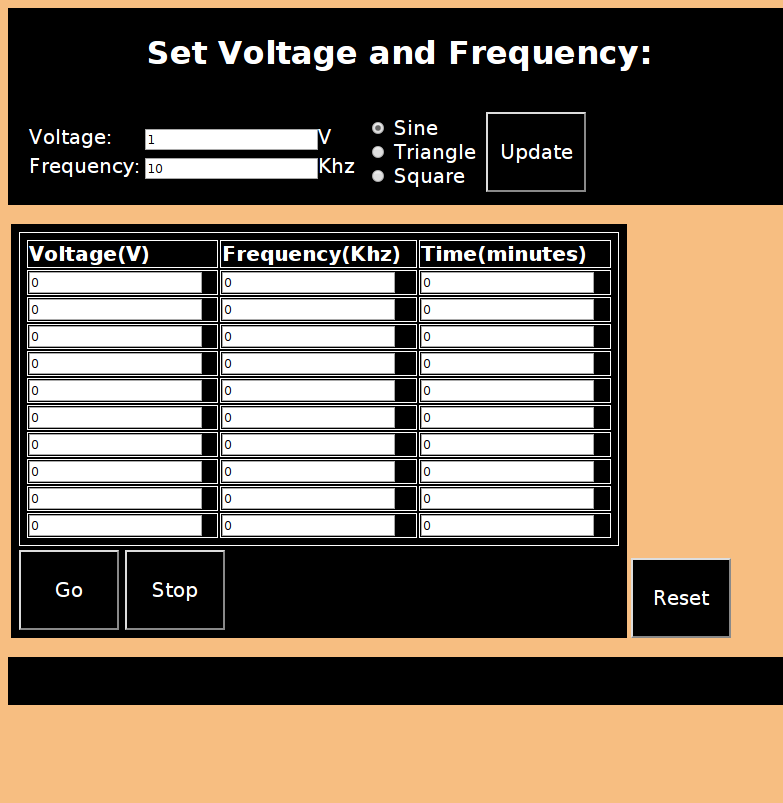
\includegraphics[width=1.0\textwidth,keepaspectratio]{491_web_interface_good.png}
\end{center}
\caption{Web Interface}
\end{figure}

\begin{figure}[!hbt]
\begin{center}
\includegraphics[width=1.0\textwidth,keepaspectratio]{"Diagram - Pi to Minigen and MCP4131"}
\end{center}
\caption{Raspberry Pi Connection Scheme}
\end{figure}

\begin{figure}[!hbt]
\begin{center}
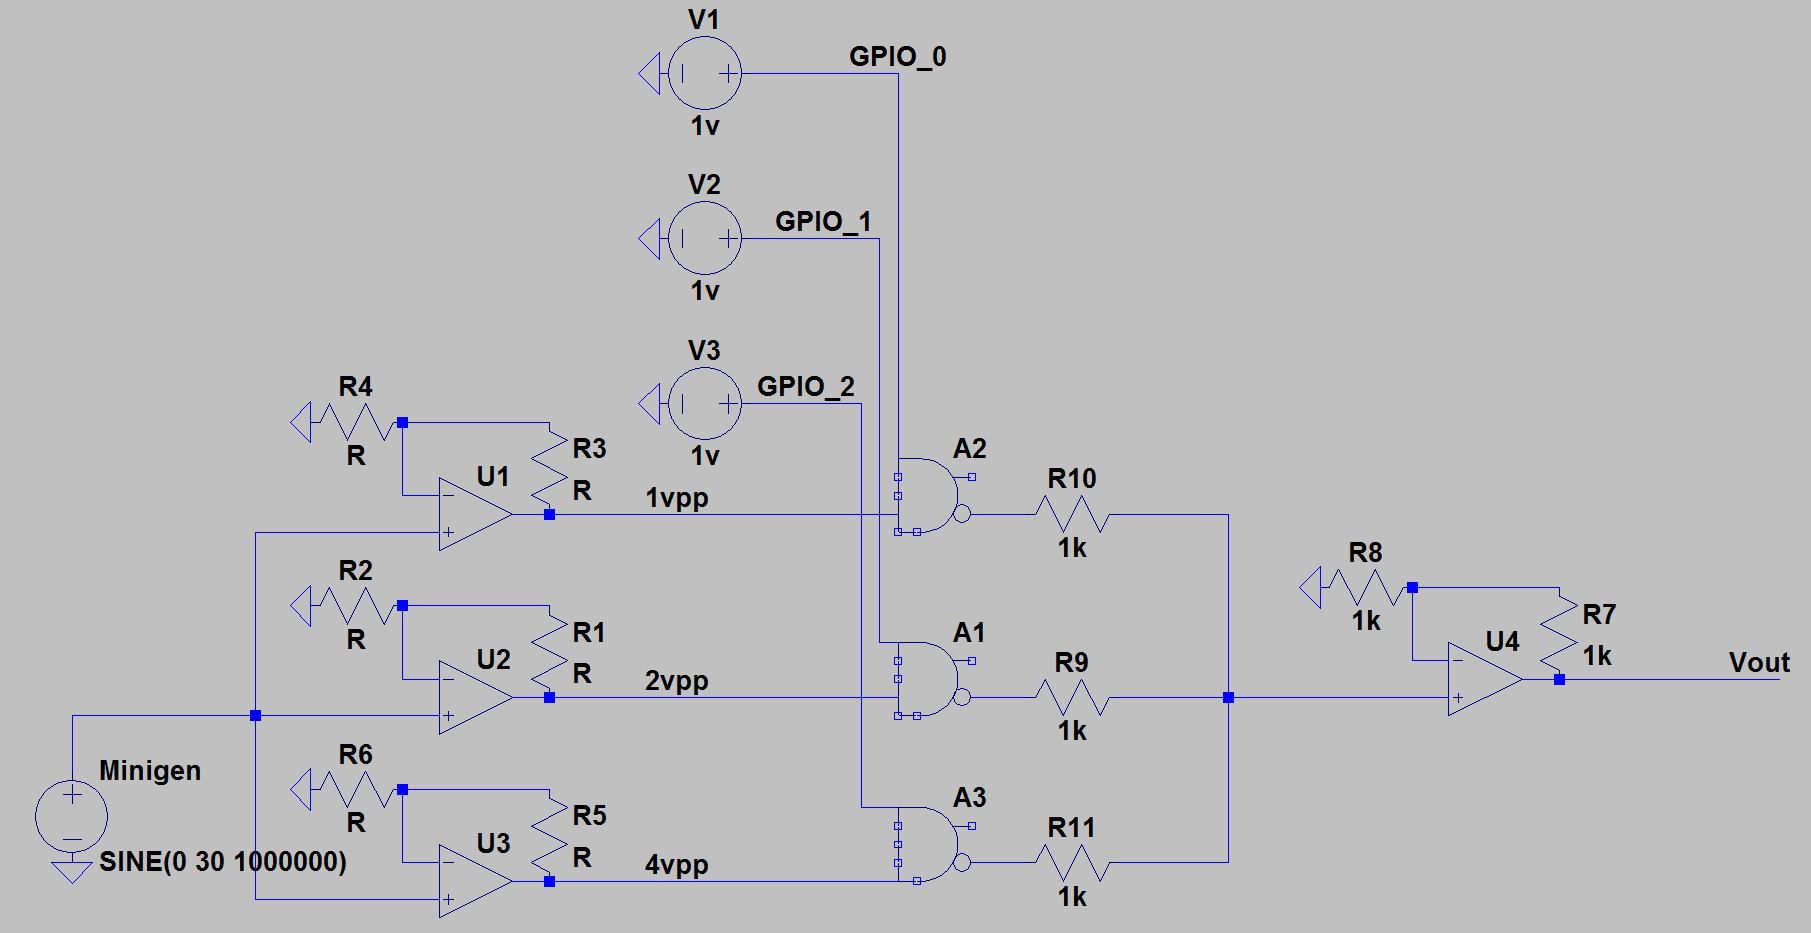
\includegraphics[width=1.0\textwidth,keepaspectratio]{voltage_control_circuit.png}
\end{center}
\caption{Voltage Control Circuit}
\end{figure}

%\subsection{Code Listing - HTML}
%\lstinputlisting[caption=Main HTML Page]{../www/index.html}

%\subsection{Code Listing - CGI Scripts}
% use listinputlisting to list files
%\lstinputlisting[caption=Update Website Script]{../cgi-bin/update.py}
%\lstinputlisting[caption=Update Voltage and Frequency Script]{../cgi-bin/update_voltage_frequency.py}
%\lstinputlisting[caption=Voltage Control Script]{../cgi-bin/voltageControl.py}
%\lstinputlisting[caption=Voltage Control Script]{../cgi-bin/voltage_regulator.py}
%\lstinputlisting[caption=Minigen Control Script]{../cgi-bin/minigen.py}
%\lstinputlisting[caption=PGA Control Script]{../cgi-bin/pga.py}
%\lstinputlisting[caption=Reset Script]{../cgi-bin/reset.py}

%\bibliographystyle{unsrt}	% Order by citation
%\bibliography{report}

\end{document}


